\chapter{What Probability Can and Cannot Do}\label{ch:01}

In January 1967 Robert Langlands, then a young mathematician at Princeton, wrote a letter of seventeen handwritten pages to Andr\'e Weil \cite{langlands1967}. In a covering note he asked Weil to read it as speculation; the letter set out conjectures that would organise much of number theory for the next six decades. Weil had it typed, the typed copy circulated widely, and its ideas were developed in Langlands' lectures \emph{Problems in the theory of automorphic forms} \cite{langlands1970}. This book asks a narrow question about that programme: what can probability theory say about it? The answer has two parts. No probabilistic method now known proves the central conjectures, and in Section~\ref{sec:01limits} we prove that no argument that sees only the limiting distribution of Frobenius data can. But the conjectures make sharp probabilistic predictions, many of those predictions are theorems that can be measured in data, and they connect to classical objects of probability: random walks on trees, Haar measure on compact groups, infinitely divisible laws, extreme values and Bayes factors.

\section{Reciprocity before Langlands}

The prehistory of the programme is the theory of reciprocity laws. Gauss' law of quadratic reciprocity says that whether a prime $q$ is a square modulo an odd prime $p\ne q$ depends only on $p$ modulo $4q$. Equivalently, whether $p$ splits in the quadratic field $\Q(\sqrt q)$ is decided by a congruence condition on $p$. Artin's reciprocity law, proved in 1927 \cite{artin1927}, extends this to every abelian extension of number fields. Over $\Q$ it says that if $F/\Q$ is abelian and $p$ is unramified in $F$, then the Frobenius element $\Frob_p\in\Gal(F/\Q)$, which records how $p$ splits in $F$, is determined by $p$ modulo the conductor of $F$. By the Kronecker Weber theorem $F$ lies in a cyclotomic field $\Q(\zeta_N)$, and $\Frob_p$ is the image of $p\bmod N$ under $(\Z/N\Z)^\times\cong\Gal(\Q(\zeta_N)/\Q)\to\Gal(F/\Q)$.

The analytic side begins with Dirichlet and Hecke. A character of $\Gal(F/\Q)$ defines an Artin $L$ function, an Euler product over primes; Artin reciprocity identifies it with a Dirichlet $L$ function $L(s,\chi)=\sum\chi(n)n^{-s}$, which has analytic continuation and a functional equation. Hecke proved the same properties for the $L$ functions of Gr\"ossencharacters of number fields, and in the 1930s built the theory of Hecke operators and Euler products for modular forms that is the subject of Chapter~\ref{ch:02} \cite{hecke1937}. Tate's thesis of 1950 recast Hecke's work on Gr\"ossencharacters in the language of harmonic analysis on adeles \cite{tate1967}, the language Langlands would use.

What is the nonabelian analogue? If $\Gal(F/\Q)$ is not abelian, $\Frob_p$ is only defined up to conjugacy, and no congruence condition on $p$ determines it. Langlands' proposal was that the correct replacement for a congruence condition is an automorphic form: the conjugacy class of $\Frob_p$ under an $n$ dimensional representation of the Galois group should match the Hecke eigenvalues at $p$ of an automorphic representation of $\GL_n$. For $n=1$ this is Artin reciprocity. For $n=2$ the best known instance is the modularity of elliptic curves, the Taniyama Shimura Weil conjecture: for every elliptic curve $E$ over $\Q$ there is a weight two newform $f$ with $L(s,E)=L(s,f)$. Taniyama raised a version of this question in 1955, Shimura sharpened it, and Weil, in the 1967 paper that proved his converse theorem \cite{weil1967}, gave it a precise and testable form by predicting that the level of $f$ equals the conductor of $E$. Wiles, with Taylor, proved it for semistable curves in 1995 \cite{wiles1995,taylorwiles1995}, which was enough for Fermat's last theorem, and Breuil, Conrad, Diamond and Taylor completed the proof for all elliptic curves over $\Q$ \cite{bcdt2001}.

\index{reciprocity}\index{Langlands programme}
The local Langlands correspondence for $\GL_n$ over $p$ adic fields was proved by Harris and Taylor and by Henniart \cite{harristaylor2001,henniart2000}. The fundamental lemma, a family of identities between orbital integrals on a group and on its endoscopic groups that is needed to stabilise the Arthur Selberg trace formula, was formulated by Langlands and Shelstad and proved by Ng\^o \cite{ngo2010}. Newton and Thorne proved symmetric power functoriality for holomorphic modular forms \cite{newtonthorne2021,newtonthorne2021b}. In 2024 Gaitsgory, Raskin and their collaborators announced a proof of the unramified global geometric Langlands conjecture in a series of long preprints \cite{gaitsgory2024}; it is a categorical statement about sheaves on the moduli space of bundles on a curve over a field of characteristic zero, and it does not by itself settle the conjectures over number fields. The general conjectures of reciprocity and functoriality over number fields remain open, and nothing in this book changes that.

\section{The conjectures for a probabilist}

We state the conjectures only to the precision needed later; Chapters~\ref{ch:02} and \ref{ch:03} develop the objects and record which cases are known. Readers who want a survey from the arithmetic side should consult Gelbart \cite{gelbart1984} and Arthur \cite{arthur2003}.

An \emph{automorphic representation} $\pi$ of $\GL_n$ over $\Q$ is, roughly, an irreducible representation of the adelic group $\GL_n(\A)$ occurring in a space of functions on $\GL_n(\Q)\backslash\GL_n(\A)$. It factors as a restricted tensor product $\pi=\bigotimes_v\pi_v$ over places $v$. At all but finitely many primes $p$ the component $\pi_p$ is \emph{unramified}, and by the Satake isomorphism an unramified representation of $\GL_n(\Q_p)$ is determined by a semisimple conjugacy class
\[
A_p(\pi)\in\GL_n(\C),
\]
its \emph{Satake parameter}. We normalise $A_p(\pi)$ unitarily, so that for cuspidal $\pi$ the Ramanujan conjecture says that its eigenvalues have absolute value one. The standard $L$ function is the Euler product $L(s,\pi)=\prod_p\det(I-A_p(\pi)p^{-s})^{-1}$, with suitable factors at the ramified primes.

On the Galois side, let $\rho:\Gal(\overline{\Q}/\Q)\to\GL_n(\overline{\Q}_\ell)$ be a continuous representation that is unramified outside a finite set and comes from geometry, for instance the action on the $\ell$ adic cohomology of a variety. For unramified $p\neq\ell$ the matrix $\rho(\Frob_p)$ is defined up to conjugacy. Fix an isomorphism $\iota:\overline{\Q}_\ell\cong\C$.

\begin{conjecture}[Reciprocity]\index{reciprocity conjecture}
For every irreducible geometric $\rho$ of dimension $n$ there is a cuspidal automorphic representation $\pi$ of $\GL_n(\A)$ such that, for all but finitely many $p$, the characteristic polynomial of $\rho(\Frob_p)$, transported to $\C$ by $\iota$, equals that of $A_p(\pi)$, after a fixed normalisation of weights.
\end{conjecture}

Functoriality is the second pillar. To a reductive group $G$ over $\Q$ Langlands attached a complex dual group $\widehat G$ and an $L$ group ${}^LG$, a semidirect product of $\widehat G$ with a Galois or Weil group that may be replaced by $\widehat G$ when $G$ is split, and to the unramified components of automorphic representations of $G$ Satake parameters, semisimple conjugacy classes in ${}^LG$.

\begin{conjecture}[Functoriality]\index{functoriality}
Let $G,H$ be reductive groups over $\Q$ with $G$ quasisplit, and $r:{}^LH\to{}^LG$ an admissible homomorphism of $L$ groups. For each automorphic representation $\pi$ of $H$ there is an automorphic representation $\Pi$ of $G$ with $A_p(\Pi)=r(A_p(\pi))$ for almost all $p$.
\end{conjecture}

The case most used in this book is $H=\GL_2$, $G=\GL_{n+1}$, $r=\Sym^n$, the $n$th symmetric power. Newton and Thorne proved it for every $n$ when $\pi$ comes from a holomorphic newform of weight at least two without complex multiplication \cite{newtonthorne2021,newtonthorne2021b}; for forms with complex multiplication it reduces to automorphic induction from Hecke characters. For general cuspidal $\pi$, Maass forms included, it is known for $n\le4$ \cite{gelbartjacquet1978,kimshahidi2002,kimsarnak2003} and open for $n\ge5$.

\subsection{The probabilistic shadow}

Take a holomorphic newform $f$ of weight $k\ge2$ with trivial character and without complex multiplication, for instance Ramanujan's $\Delta$ or the weight two form attached to an elliptic curve over $\Q$ without complex multiplication. For $p$ not dividing the level, normalise its Hecke eigenvalue at $p$ to $x_p=a_p/p^{(k-1)/2}$. By Deligne's theorem \cite{deligne1974} $x_p\in[-2,2]$, so $x_p=2\cos\theta_p$ for an angle $\theta_p\in[0,\pi]$, and the unitarily normalised Satake parameter is the conjugacy class of $\mathrm{diag}(e^{i\theta_p},e^{-i\theta_p})$ in the compact group $\SU(2)$.

\begin{definition}\index{equidistribution}
Let $K$ be a compact group with normalised Haar measure $h$, and let $\pi(x)$ be the number of primes $p\le x$ (context distinguishes this function from an automorphic representation $\pi$). A sequence $(g_p)$ of conjugacy classes in $K$ indexed by primes is \emph{equidistributed} with respect to Haar measure if $\pi(x)^{-1}\sum_{p\le x}\phi(g_p)\to\int_K\phi\,dh$ as $x\to\infty$ for every continuous class function $\phi$ on $K$.
\end{definition}

For $K=\SU(2)$ a class function is a function of the trace $x=2\cos\theta$, and the image of Haar measure under the trace is the semicircle law
\[
\ST(dx)=\frac{1}{2\pi}\sqrt{4-x^2}\,dx\qquad\text{on }[-2,2],
\]
whose even moments $\int x^{2m}\,d\ST$, $m=1,2,3,\dots$, are the Catalan numbers $1,2,5,14,42,\dots$, as for Wigner's semicircle law for large random matrices.

\begin{theorem}[Sato Tate; Barnet Lamb, Geraghty, Harris, Taylor]\label{thm:01satotate}\index{Sato Tate law}
For every holomorphic newform of weight $k\ge2$ with trivial character and without complex multiplication, the normalised eigenvalues $x_p$ are equidistributed with respect to $\ST$.
\end{theorem}

The conjecture was formulated by Sato and Tate in the 1960s \cite{tate1965}. For elliptic curves over totally real fields with nonintegral $j$ invariant it was proved through potential automorphy by Clozel, Harris, Shepherd Barron and Taylor \cite{cht2008,taylor2008,hsbt2010}, and for all newforms as in the theorem, which include the form of every elliptic curve over $\Q$ without complex multiplication, by Barnet Lamb, Geraghty, Harris and Taylor \cite{blght2011}. The argument, due in outline to Serre \cite{serre1968}, is short once the hard input is available. The traces of the irreducible representations of $\SU(2)$ are $\tr\Sym^n=U_n(x/2)$, with $U_n$ the Chebyshev polynomials of the second kind, and by the Peter Weyl theorem equidistribution is equivalent to $\pi(x)^{-1}\sum_{p\le x}U_n(x_p/2)\to0$ for every $n\ge1$. That vanishing follows by a Tauberian theorem from holomorphy and nonvanishing of $L(s,\Sym^nf)$ on the line $\Re s=1$, which is what (potential) automorphy of $\Sym^nf$ provides. Chapter~\ref{ch:04} gives the argument in full.

Functoriality is the \emph{input}; equidistribution is the \emph{output}. In general the Langlands conjectures predict the following.

\begin{quote}
\emph{Normalised Frobenius conjugacy classes are equidistributed with respect to Haar measure on a compact group, the Sato Tate group, attached to the motive or automorphic representation.}
\end{quote}

This prediction is the probabilistic shadow of the Langlands conjectures, and it is concrete and testable. Figure~\ref{fig:satotate} shows it for two elliptic curves. For $E_1:y^2=x^3+x+1$, which has discriminant $-496$, conductor $496$ and no complex multiplication, we computed $a_p=p+1-\#E_1(\mathbb{F}_p)$ for all $664{,}577$ good primes below $10^7$ with PARI/GP. The histogram of $x_p=a_p/\sqrt p$ sits on the semicircle and its even moments approach $1,2,5,14,42,132$. For $E_2:y^2=x^3-x$, which has complex multiplication by $\Z[i]$ and conductor $32$, the primes $p\equiv3\bmod4$ are supersingular, with $a_p=0$, and for $p\equiv1\bmod4$ the angles $\theta_p$ are uniformly distributed on $[0,\pi]$ by Hecke's theorem \cite{hecke1918}; the law is
\[
\mu_{\mathrm{CM}}=\tfrac12\delta_0+\tfrac12\,\frac{dx}{\pi\sqrt{4-x^2}},
\]
the image of Haar measure on the normaliser of a maximal torus in $\SU(2)$, with even moments $\tfrac12\binom{2m}{m}=1,3,10,35,126,462$ for $m=1,\dots,6$. Among the good primes below $4\times10^4$ the fraction with $a_p=0$ is $0.5038$.

\begin{figure}[t]
\centering
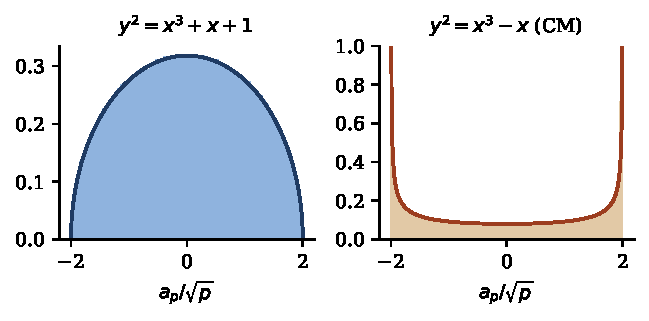
\includegraphics[width=\textwidth]{figs/satotate.pdf}
\caption{Normalised Frobenius traces $a_p/\sqrt p$ for all good primes below $10^7$. Left: $E_1:y^2=x^3+x+1$, histogram of all traces against the Sato Tate density $\sqrt{4-x^2}/(2\pi)$. Right: $E_2:y^2=x^3-x$, which has complex multiplication; histogram of the nonzero traces (the primes $p\equiv1\bmod4$), scaled to their share of all good primes (about $\tfrac12$), against the continuous part $1/(2\pi\sqrt{4-x^2})$ of $\mu_{\mathrm{CM}}$, which has mass $\tfrac12$. The atom of mass $\tfrac12$ at zero, from the primes $p\equiv3\bmod4$, is not drawn.}\label{fig:satotate}
\end{figure}

The two histograms distinguish two compact groups: the Sato Tate group of $E_1$ is $\SU(2)$, and that of $E_2$ is the normaliser $N(\mathrm{U}(1))$ of the diagonal torus. Telling them apart from data is a statistical problem, the subject of Chapter~\ref{ch:12}.

\section{A map of methods}

Table~\ref{tab:01map} lists the main families of probabilistic and computational methods that touch the programme, the target in each case, and what each delivers. ``Proves'' means the method is the engine of a theorem, usually with arithmetic input supplied from elsewhere. ``Reformulates'' means it recasts a conjecture as an equivalent probabilistic statement. ``Tests'' means it produces evidence, calibration or conjectural constants. ``None known'' means that no contribution is known.

\begin{table}[t]
\centering\small
\begin{tabular}{p{1.4in}p{1.4in}p{1.3in}}
\toprule
Method & Langlands target & Status\tabularnewline
\midrule
\raggedright Weyl criterion, moments & \raggedright Sato Tate and general Sato Tate laws & \raggedright proves, given functoriality\tabularnewline
\raggedright Tauberian theorems & \raggedright Prime number theorems for $L(s,\Sym^n\pi)$ & \raggedright proves, given automorphy\tabularnewline
\raggedright Random walks on trees & \raggedright $p$ adic Plancherel measure, Hecke operators & \raggedright proves\tabularnewline
\raggedright Trace formula as expectation & \raggedright Vertical Sato Tate \cite{serre1997,cdf1997} & \raggedright proves\tabularnewline
\raggedright Random walks on isogeny graphs & \raggedright Kemeny constants, spanning trees, mixing & \raggedright proves (Part~III and Chapter~\ref{ch:hit})\tabularnewline
\raggedright Random matrix theory & \raggedright Low lying zeros \cite{katzsarnak1999,ils2000} & \raggedright proves for restricted support (often under GRH), tests beyond\tabularnewline
\raggedright Interlacing, random graphs & \raggedright Bipartite Ramanujan graphs \cite{mss2015} & \raggedright proves\tabularnewline
\raggedright L\'evy and Thorin measures & \raggedright Positivity, Riemann hypothesis and Artin conjecture reformulations; squarefree integers (Chapter~\ref{ch:squarefree}); the steps of the proof of Fermat's last theorem (Chapter~\ref{ch:flt}); inversions between Frobenius traces, P\'olya kernels and zeros (Chapter~\ref{ch:lap}) & \raggedright reformulates, tests; proves identities (Chapters~\ref{ch:squarefree} and \ref{ch:lap})\tabularnewline
\raggedright Poisson Dirichlet law, Dirichlet processes & \raggedright Chebotarev densities in the prime factors of random integers, Mertens constants per class (Chapter~\ref{ch:pd}) & \raggedright proves\tabularnewline
\raggedright Extreme values & \raggedright $L$ values of eta products & \raggedright proves identities\tabularnewline
\raggedright Bayesian model choice & \raggedright Sato Tate group identification & \raggedright proves consistency, given equidistribution\tabularnewline
\raggedright Point counting, modular symbols & \raggedright Data for all of the above & \raggedright tests\tabularnewline
\raggedright Any of the above & \raggedright Reciprocity, functoriality & \raggedright no proof known\tabularnewline
\bottomrule
\end{tabular}
\caption{Probabilistic and computational methods in the Langlands programme, and what each delivers.}\label{tab:01map}
\end{table}

The last line of the table is the subject of the next section.

\section{The key limitation}\label{sec:01limits}

Could one prove reciprocity probabilistically, by showing that some sequence of Galois data has the statistics that automorphy forces? The following proposition shows that the limiting empirical law of the data cannot do it.

Let $\mathcal P$ be the set of primes. A set $S\subset\mathcal P$ has \emph{density zero} if $\#\{p\le x:p\in S\}/\pi(x)\to0$. Say that a sequence $(x_p)_{p\in\mathcal P}$ of real numbers \emph{comes from} a cuspidal automorphic representation $\pi$ of $\GL_2(\A)$ with trivial central character if $x_p=\tr A_p(\pi)$ for all but finitely many primes $p$, and call it \emph{automorphic} if it comes from some such $\pi$. Both notions are unchanged when finitely many terms are changed. A sequence $(x_p)\in[-2,2]^{\mathcal P}$ is equidistributed with respect to $\ST$ if $\pi(x)^{-1}\sum_{p\le x}\phi(x_p)\to\int\phi\,d\ST$ for every continuous $\phi$ on $[-2,2]$.

\begin{proposition}[Equidistribution does not determine automorphy; this book]\label{prop:01limits}\index{strong multiplicity one}
Let $\mathcal E$ be the set of sequences $(x_p)\in[-2,2]^{\mathcal P}$ that are equidistributed with respect to $\ST$.
\begin{enumerate}
\item $\mathcal E$ has the cardinality of the continuum and contains continuum many sequences no two of which agree at all but finitely many primes. The automorphic sequences fall into countably many classes under the relation of agreeing at all but finitely many primes, so all but countably many of those sequences are not automorphic.
\item Let $(x_p)\in[-2,2]^{\mathcal P}$ come from $\pi$, and let $(x'_p)\in[-2,2]^{\mathcal P}$ differ from $(x_p)$ exactly on an infinite set $S$ of density zero. Then $(x'_p)$ is not automorphic, and $(x'_p)\in\mathcal E$ if and only if $(x_p)\in\mathcal E$.
\end{enumerate}
\end{proposition}

\begin{proof}
We first show that density zero alterations do not change limits of empirical averages. Let $(x_p),(x'_p)\in[-2,2]^{\mathcal P}$ agree outside a density zero set $S$, and let $\phi$ be continuous on $[-2,2]$. Then
\[
\Bigl|\frac1{\pi(x)}\sum_{p\le x}\phi(x'_p)-\frac1{\pi(x)}\sum_{p\le x}\phi(x_p)\Bigr|\le 2\|\phi\|_\infty\,\frac{\#\{p\le x:p\in S\}}{\pi(x)}\longrightarrow0,
\]
so either both empirical averages converge, to the same limit, or neither does. In particular $(x'_p)\in\mathcal E$ if and only if $(x_p)\in\mathcal E$.

(1) By Theorem~\ref{thm:01satotate} the normalised eigenvalues $x_p=\tau(p)/p^{11/2}$ of $\Delta$ form an element of $\mathcal E$. Let $S$ be an infinite set of density zero, for instance $S=\{p_{k^2}:k\ge1\}$, where $p_j$ is the $j$th prime; it has $\lfloor\pi(x)^{1/2}\rfloor$ elements up to $x$. For $c\in[-2,2]$ let $(x^{(c)}_p)$ equal $c$ on $S$ and agree with $(x_p)$ off $S$. By the first paragraph each $(x^{(c)}_p)$ lies in $\mathcal E$, and for $c\ne c'$ the sequences $(x^{(c)}_p)$ and $(x^{(c')}_p)$ differ at every prime of the infinite set $S$. These are continuum many elements of $\mathcal E$, no two agreeing at all but finitely many primes, and $|\mathcal E|\le|[-2,2]^{\mathcal P}|=2^{\aleph_0}$.

On the other side, every cuspidal automorphic representation $\pi$ of $\GL_2(\A)$ has nonzero vectors fixed by some open compact subgroup $K$ of $\GL_2(\A_f)$. There are countably many such $K$, since each contains some principal congruence subgroup $K(N)$, is a finite union of cosets of $K(N)$, and $\GL_2(\A_f)/K(N)$ is countable. For fixed $K$, the cuspidal functions on $\GL_2(\Q)Z(\A)\backslash\GL_2(\A)$ that are right invariant under $K$ form a separable Hilbert space on which $\GL_2(\R)$ and the Hecke operators of level $K$ act with discrete spectrum and finite multiplicities, and each $\pi$ with trivial central character and nonzero $K$ fixed vectors occurs in it; so there are countably many such $\pi$. Hence there are countably many $\pi$ in all, and the sequences that come from a given $\pi$ form a single class under agreement at all but finitely many primes. A class contains at most one of the sequences $(x^{(c)}_p)$, so all but countably many of them are not automorphic.

(2) The second assertion was proved in the first paragraph. Suppose $(x'_p)$ came from some $\pi'$. Then $\tr A_p(\pi')=x'_p=x_p=\tr A_p(\pi)$ for all primes outside $S\cup F$, with $F$ finite, and $S\cup F$ has natural density zero, hence Dirichlet density zero. Ramakrishnan's refinement of strong multiplicity one \cite{ramakrishnan1994} states that two cuspidal automorphic representations of $\GL_2(\A)$ with trivial central character are isomorphic if their Hecke eigenvalues $\tr A_p$ agree at all primes outside a set of density less than $1/8$. Therefore $\pi'\cong\pi$, and hence $x'_p=\tr A_p(\pi)=x_p$ for all but finitely many $p$. This contradicts the hypothesis that the sequences differ at every prime of the infinite set $S$.
\end{proof}

\begin{corollary}[this book]\label{cor:01functional}
Let $\Phi$ be any function on $[-2,2]^{\mathcal P}$ that is unchanged when a sequence is altered on a set of density zero; for instance any function of the set of weak limit points of the empirical measures $\pi(x)^{-1}\sum_{p\le x}\delta_{x_p}$ as $x\to\infty$, which by the first paragraph of the proof above is unchanged by such alterations. Then for every automorphic $(x_p)\in[-2,2]^{\mathcal P}$ there are continuum many sequences in $[-2,2]^{\mathcal P}$ that are not automorphic and on which $\Phi$ takes the value it takes on $(x_p)$; if $(x_p)\in\mathcal E$, they all lie in $\mathcal E$. In particular $\Phi$ cannot characterise automorphy.
\end{corollary}

\begin{proof}
Fix an infinite set $S$ of density zero and apply part (2) of Proposition~\ref{prop:01limits} to every $(x'_p)\in[-2,2]^{\mathcal P}$ that agrees with $(x_p)$ off $S$ and differs from it at every prime of $S$. There are continuum many such sequences, since each $x'_p$ with $p\in S$ ranges over $[-2,2]\setminus\{x_p\}$; none is automorphic, and $\Phi$ takes the same value on all of them and on $(x_p)$.
\end{proof}

Any argument that uses only the limiting distribution of Frobenius traces therefore sees the same object for an automorphic representation and for continuum many nonautomorphic impostors. Rates of convergence do not help either. If $\epsilon(x)\pi(x)\to\infty$, there is an infinite set $S$ with $\#\{p\le x:p\in S\}\le\epsilon(x)\pi(x)$ for all $x$, and an alteration on $S$ changes every empirical average $\pi(x)^{-1}\sum_{p\le x}\phi(x_p)$ by at most $2\|\phi\|_\infty\epsilon(x)$. With $\epsilon(x)=\pi(x)^{-3/4}$, for instance, which satisfies both $\epsilon(x)\pi(x)\to\infty$ and $\epsilon(x)=o(\pi(x)^{-1/2})$, this gives impostors that the discrepancy statistics of Chapter~\ref{ch:05}, which live at the scale $\pi(x)^{-1/2}$, cannot see. What distinguishes the genuine sequence is structure that couples different primes: the analytic continuation and functional equation of the Dirichlet series built from it and of all its twists, and the Galois representation attached to it, which for an elliptic curve makes each $a_p=\sqrt p\,x_p$ an integer whose residue modulo a prime $\ell\ne p$ is determined by the Frobenius class of $p$ in the field generated by the $\ell$ torsion points. Converse theorems, from Weil \cite{weil1967} to Cogdell and Piatetski Shapiro \cite{cogdellps1994}, characterise automorphy through the first kind of coupling; modularity lifting theorems, from Wiles onward \cite{wiles1995,taylorwiles1995}, establish it through the second, by Galois deformation theory and congruences between automorphic forms. No probabilistic method currently exploits either. Chapter~\ref{ch:recip} restates part of the first kind of coupling as a symmetry of functions computed from Frobenius traces, the conductor and the gamma factor, and that part together with the generalized Riemann hypothesis as a positivity property of such functions; this is a reformulation, not a method of proof. Probability therefore enters the programme through consequences of the conjectures, as a calibration tool and as a source of reformulations, not as a proof technique for reciprocity itself.

\begin{remark}
The same argument applies to any statistic that is a limit of averages over primes in which each prime carries weight $O(1/\pi(x))$, for instance the empirical joint law of consecutive traces $(x_{p_n},x_{p_{n+1}})$. It says nothing about statistics that weight individual primes heavily, or that use the analytic properties of the full Dirichlet series and its twists. A sparser alteration, on an infinite set $S$ with $\sum_{p\in S,\,p\le x}\log p=o(\sqrt x)$, moves every twisted sum $\sum_{p\le x}x_p\chi(p)\log p$ by $o(\sqrt x)$, so properties of these sums at the square root scale cannot characterise automorphy either; whether, uniformly over characters $\chi$ of growing conductor, they can decide closeness to a newform is Open Problem~\ref{op:inverse} of Chapter~\ref{ch:13}.
\end{remark}

\section{What the methods deliver}

Within these limits there is a great deal to prove. The book is organised in five parts.

\subsection{Part I: Foundations}
Chapter~\ref{ch:02} develops modular forms, Hecke operators, Euler products and functional equations for readers trained in probability, and isolates two facts used throughout: normalised Hecke eigenvalues are traces of elements of $\SU(2)$, and the completed $L$ function of $\Delta$ is the Mellin transform of a positive function. Chapter~\ref{ch:03} treats Galois representations and the Chebotarev density theorem, reciprocity, the dual group and the Satake isomorphism, functoriality and the Sato Tate group, and records which cases are known. Appendix~\ref{app:A} collects the probability used later.

\subsection{Part II: Equidistribution}
The Weyl criterion on compact groups turns equidistribution into the vanishing of averages of characters. For $\SU(2)$ these are Chebyshev polynomials, and for the CM law $\mu_{\mathrm{CM}}$ the averages $\int U_n(x/2)\,d\mu_{\mathrm{CM}}$ equal $1$ when $4\mid n$ and $0$ otherwise, a fingerprint of the Sato Tate group. Chapter~\ref{ch:04} gives Serre's derivation of Sato Tate from symmetric power functoriality. Chapter~\ref{ch:05} studies the rate of convergence (the discrepancy $D_n$ of the first $n$ traces, which for our curves sits at the scale $n^{-1/2}$ of independent sampling), the bias of the weighted sums $\sum_{p\le x}a_p\log p/p$, which through the explicit formula and under the Riemann hypothesis for $L(s,E)$ encodes the analytic rank of an elliptic curve in logarithmic mean, and the Lang Trotter conjecture on how often $a_p$ takes a fixed value.

Chapter~\ref{ch:06} turns to the other random matrix limit, in which the dimension of the group tends to infinity and eigenvalues model zeros of $L$ functions: the pair correlation of Montgomery and Dyson, the symmetry types of Katz and Sarnak, low lying zeros of families of modular forms and the moment conjectures of Keating and Snaith. Chapter~\ref{ch:06b} finds the same semicircle in Kloosterman sums, through Katz's vertical Sato Tate theorem \cite{katz1988} and the random Fourier series of Kowalski and Sawin \cite{kowalskisawin2016}. Chapter~\ref{ch:06c} replaces Haar random elements of a compact group by random finite abelian groups: the Cohen Lenstra heuristics for class groups and the Poonen Rains model for Selmer groups, with what they predict for ranks, compared with class groups and Selmer groups computed for this book.

\subsection{Part III: Random walks and hitting times}
Hecke operators, suitably normalised, are Markov operators. The Bruhat Tits tree of the group $\PGL_2(\Q_q)$ is the $(q+1)$ regular tree, $T_q$ acts as its adjacency operator, and the spectral measure of simple random walk on the tree is the Kesten McKay law \cite{kesten1959,mckay1981}, which is also the $q$ adic Plancherel measure. Chapter~\ref{ch:07} shows that its Chebyshev moments are $q^{-n/2}$ for even $n$ and $0$ for odd $n$, and that it converges to the semicircle as $q\to\infty$, which explains heuristically, but does not prove, why the horizontal Sato Tate law (one form, the prime varying) and the vertical one (one prime, the form varying) are compatible. Chapter~\ref{ch:08} turns to finite quotients, whose Ihara zeta functions make the Ramanujan property a graph Riemann hypothesis, and to the supersingular isogeny graphs of Pizer \cite{pizer1990}, on which the Ramanujan bound for Hecke eigenvalues of weight two forms becomes an optimal spectral gap. We prove that the Kemeny constant of the supersingular $\ell$ isogeny graph, the expected time to hit a target drawn from the stationary distribution, is asymptotic to $\ell/(\ell-1)$ times the number of vertices.

\subsection{Part IV: L\'evy and Thorin measures}
Chapter~\ref{ch:09} starts from Khinchine's observation that for $\sigma>1$ the function $t\mapsto\zeta(\sigma+it)/\zeta(\sigma)$ is the characteristic function of an infinitely divisible law. For an automorphic $L$ function the corresponding L\'evy Khintchine exponent has weights of both signs, and positivity returns for Rankin Selberg $L$ functions: for $\sigma>1$, $t\mapsto L(\sigma+it,\pi\times\tilde\pi)/L(\sigma,\pi\times\tilde\pi)$ is again the characteristic function of an infinitely divisible law. Chapter~\ref{ch:09b} follows $\log|L|$ on the critical line, through Selberg's central limit theorem, the log correlated field of Fyodorov, Hiary and Keating and its maximum, and multiplicative chaos, tested on $L(s,\Delta)$.

For Ramanujan's $\Delta$ the completed $L$ function $\Lambda(s,\Delta)$ is the Mellin transform of the positive function $y\mapsto\Delta(iy)$, so $\Lambda(6+it)/\Lambda(6)$ is the characteristic function of a symmetric random variable, and the Riemann hypothesis for $\Delta$ says that this characteristic function has only real zeros. In Chapter~\ref{ch:10} we prove that the Riemann hypothesis for $\Delta$ is equivalent to $s\mapsto\Lambda(6)/\Lambda(6+\sqrt s)$ being the Laplace transform of a generalized gamma convolution in the sense of Thorin and Bondesson \cite{thorin1977,bondesson1992}, with Thorin measure carried by the squared ordinates of the zeros. This is a reformulation, not a proof. Chapters~\ref{ch:10b} and \ref{ch:10c}, extending the first author's earlier work \cite{polson2018vdp}, turn it into a framework. For every cuspidal automorphic representation of $\GL_n$ over $\Q$ the generalized Riemann hypothesis is equivalent to the Thorin property, to complete monotonicity of a L\'evy function built from the zeros, and to positive semidefiniteness of Hankel matrices of power sums computable from the central Taylor coefficients alone; the order of vanishing at the centre, which for an elliptic curve is the Mordell Weil rank under the conjecture of Birch and Swinnerton Dyer, appears as a degenerate Thorin atom at the origin of mass half the order. Locally the Ramanujan conjecture at a prime is exactly a Thorin property of the Euler factor, and the framework becomes unconditional for curves over finite fields, for Ramanujan graphs, including the supersingular isogeny graphs, and for Hecke random walks on Bruhat Tits trees, whose passage times are generalized gamma convolutions with explicit large deviations. Chapter~\ref{ch:10d} recasts all of this, as in \cite{polson2018vdp}, as van Dantzig pairs and Wald couples, proves the sine squared transport from Euler products to Thorin densities, and tests the class of Konstantopoulos, Patie and Sarkar \cite{konstantopoulospatiesarkar2024} against $L$ functions.

Chapters~\ref{ch:squarefree} to \ref{ch:scholze} test the framework on three cases. Chapter~\ref{ch:squarefree} follows the squarefree integers: their counting error is governed by the zeros of $\zeta$, the constant of the squarefree problem is a combination of two tilted means of the P\'olya law of $\xi$, a Gamma smoothing turns the error into an average of the Mertens function, and the Thorin picture extends into the critical strip and to imaginary quadratic fields, whose P\'olya kernels are positive when $|d|<\pi^2$ and take negative values whenever $2$ and $3$ are inert. Chapter~\ref{ch:beta} does the same for Dirichlet's $\beta$ function, whose kernel is built from the cube of Dedekind's eta function, and proves for $\beta$ and for $\xi$, on the lines $\operatorname{Re}s=\alpha$ with $\frac12<\alpha\le3.15$ and up to the heights to which their Riemann hypotheses are verified, that the real part of the logarithmic derivative is smallest on the real axis, which for $\xi$ Lagarias proved on every line to the right of the centre under the Riemann hypothesis, and Garunk\v{s}tis unconditionally for $\alpha\ge1$. Chapter~\ref{ch:scholze} computes signed Thorin densities by Stieltjes inversion and counts zeros numerically by the argument principle for $\zeta$, $L(s,\chi_{12})$ and $L(s,\Delta)$; its first section says where Scholze's work enters the theory of $L$ functions, and that the computations do not use it. None of the three chapters proves a Riemann hypothesis.

Chapter~\ref{ch:recip} turns these devices on reciprocity. It derives quadratic reciprocity and Gauss's sign from the characteristic function of the normal law, puts Frobenius traces and Hecke eigenvalues on one probability space, where irreducible Artin representations and cuspidal automorphic representations are both orthonormal systems of random variables, reads the Frobenius labelled prime factorisation of a random integer as a Gamma process, and restates Hecke's converse theorem at level one as a symmetry of a P\'olya kernel, and the holomorphy and the generalized Riemann hypothesis of a self dual Artin $L$ function as the complete monotonicity of a heat trace computed from Frobenius traces, the conductor and the gamma factor. These are reformulations. Finitely many evaluations of the heat trace can disprove holomorphy or the generalized Riemann hypothesis but are not known to verify them, even to a finite height, and no new case of reciprocity is proved.

Chapter~\ref{ch:hit} reads reciprocity through hitting times. For the walk on supersingular elliptic curves in characteristic $N$ along isogenies of degree $\ell$, the Kemeny constant is a harmonic sum of the factors $\ell+1-a_\ell(f)$ of $|J_0(N)(\mathbb F_\ell)|$, and for $N\equiv1\bmod12$ the number of spanning trees is $|J_0(N)(\mathbb F_\ell)|$ divided by the number of vertices, a formula of Hashimoto \cite{hashimoto1989,li2019} that Munier and Shnidman \cite{muniershnidman2023} read as a reciprocity law exchanging the two primes. Chebotarev densities become hitting rates for the largest prime factors of a random integer, the Thorin converse theorem a statement about explosion times of pure birth processes, and the functional equation of the $L$ function of an odd primitive Dirichlet character an identity between two expansions of a signed exit law of Brownian motion. These too are reformulations, and no new case of reciprocity is proved.

Chapter~\ref{ch:flt} follows the proof of Fermat's last theorem through the same language. Weight one newforms, through which the theorem of Langlands and Tunnell gives the residual modularity that Wiles's argument starts from, are exactly the newforms whose label laws are supported on finitely many points; modularity becomes, through Weil's converse theorem, a family of reflection symmetries of twisted P\'olya kernels built from point counts and the conductor; the density of the primes $\ell$ at which $p$ does not divide $|E(\mathbb F_\ell)|$, the local density of Koblitz's conjecture, becomes the shape of a Gamma law, positive for a Frey curve and $p\ge5$ by Serre's argument from Mazur's torsion theorem; and the genus zero of $X_0(2)$, which ends the proof, becomes the emptiness of a Thorin measure built from Hecke eigenvalues, or a Kemeny constant equal to zero. These are restatements: no step of the proof is reproved and no new case of modularity is proved, and the content of the proof is in the theorems of Langlands and Tunnell, Mazur, Ribet, Wiles, and Taylor and Wiles, on the curve of Hellegouarch and Frey and the reduction of Frey and Serre.

Chapter~\ref{ch:lap} collects the inverse Laplace transforms behind the earlier chapters of this part and computes with them. Bohr means invert the sine squared transport, so that the transported density of an $L$ function on any half line determines its Frobenius traces, which we recover at the primes below $64$ from the transported density of $\eta(z)\eta(23z)$. Bromwich inversion of the Artin $L$ function of $x^3-x-1$ on the critical line, computed as $\zeta_K/\zeta$, returns the weight one form; it uses the holomorphy of this $L$ function, which Hecke's identification of it with the $L$ function of the form supplies, and in general the modularity of the result is the content of Weil's converse theorem. As in \cite{polson2017}, the shifted Thorin densities of Chapter~\ref{ch:10d} form a Cauchy semigroup in the basepoint, in which each zero is seen through Cauchy noise, and by a theorem of Roynette and Yor \cite{roynetteyor2005} the Thorin variable of an Euler product with nonnegative coefficients has a Pareto tail of index $\frac32$. A last section relates atomic Thorin laws to the B splines of Curry and Schoenberg, and reads the Sato Tate law as the density that minimises the roughness penalty of Good and Gaskins among those vanishing on the walls of the alcove. Most of these results are known, and no case of reciprocity is proved.

Chapter~\ref{ch:pd} relates the Gamma process of Chapter~\ref{ch:recip} to classical laws. The normalised sizes of the prime factors of a uniform random integer follow the Poisson Dirichlet law by Billingsley's theorem, as the normalised cycle lengths of a random permutation do; normalised, the Gamma process with Frobenius labels is Ferguson's Dirichlet process, whose base measure is the Haar measure that Chebotarev's theorem gives, so that the limit of every Frobenius functional is a standard exponential variable times a Dirichlet mean; and the random integers weighted by the coefficients of the powers of $\zeta$ give the whole Ewens family, with the exponent of the singularity at $s=1$ as Ewens parameter. For a uniform random integer below $x$, the class of a size biased prime factor approaches Haar measure at rate $1/\log x$, the class of the largest one faster still, but the classes of the distinct prime factors only at rate $1/\log\log x$, with Mertens constants per class computed from $L(1,\chi)$ and $\frac{L'}L(1,\chi)$: among the distinct prime factors of random integers below $10^7$, the primes that split completely in the field of $x^3-x-1$ have less than half their Haar share. A last section asks which of Bondesson's theorems on generalized gamma convolutions do arithmetic work. These are theorems about random integers, most of them known, and no case of reciprocity is proved.

Chapter~\ref{ch:gl1} treats degree one, where reciprocity is a theorem: by Kronecker and Weber over $\Q$, by Artin's reciprocity law over a number field, and for Hecke's characters of infinite order. Dirichlet's theorem on primes in progressions becomes a Dirichlet process on the classes modulo $q$, with Mertens constants computed from $L(1,\chi)$ and with Landau's theorem on the integers that have no prime factor in a given class as the atom at zero of Chapter~\ref{ch:pd}; Hecke's theorem on the angles of Gaussian primes becomes a Dirichlet process on the circle; and the Thorin measure of a degree one $L$ function is checked against its zeros. By Deuring's theorem the $L$ function of an elliptic curve with complex multiplication is that of a Hecke character of the imaginary quadratic field, and seen from that field the Rankin Selberg subordinator of Chapter~\ref{ch:recip} is the sum of two independent copies of itself seen from $\Q$, so that the Gamma shape test of Chapter~\ref{ch:recip} detects complex multiplication, here as a theorem.

Chapter~\ref{ch:maass} turns to the Maass forms, the eigenfunctions of the hyperbolic Laplacian on the modular surface and the other half of the automorphic spectrum of $\SL_2(\Z)$. With the normalised hyperbolic area the modular surface is a probability space, and Brownian motion on it is ergodic with that law. Read as a heat trace, the Selberg trace formula of a compact hyperbolic surface says that the total return probability of Brownian motion is the free return probability plus a sum over closed geodesics, which is McKean's reading \cite{mckean1972}. Selberg's eigenvalue conjecture becomes the complete monotonicity of the heat trace over the cusp forms, as the holomorphy and the generalized Riemann hypothesis of a self dual Artin $L$ function became that of a heat trace in Chapter~\ref{ch:recip}. Weyl's law keeps the eigenvalues out of the Thorin class, while the closed geodesics, ordered by length, form a system of primes to which the sine squared transport of Chapter~\ref{ch:10d} and the Poisson Dirichlet limits of Chapter~\ref{ch:pd} apply unconditionally. A last section states the Eichler Selberg trace formula and reads it as the moment identity behind Serre's vertical Sato Tate law. These are reformulations, and no new case of Selberg's conjecture is proved.

Chapter~\ref{ch:percolation} takes up the other body of Langlands's work, on conformal invariance in critical percolation. Cardy's formula for the probability that a critical rectangle of aspect ratio $r$ is crossed from left to right is the distribution function of a $\mathrm{Beta}(\frac13,\frac13)$ law at the modular lambda function of $ir$, and the log odds of that law is an extended generalized gamma convolution with Thorin atoms at $n+\frac13$. Differentiating in $r$ gives a constant times $\eta(ir)^4$, so that the aspect ratio at which a critical rectangle stops being crossed is a random variable whose Mellin transform is, up to a constant, the completed $L$ function of the elliptic curve $y^2=x^3+1$ of conductor $36$: the modularity of the curve is what turns a percolation law into an $L$ function. The logarithm of this crossing threshold is not infinitely divisible and the threshold is not a generalized gamma convolution, but numerically it is infinitely divisible and self decomposable, the probabilistic form of the renormalisation fixed point of Langlands, Pouliot and Saint Aubin. The generalized Riemann hypothesis for the curve is equivalent to the positivity of Hankel matrices built from the cumulants of the logarithm of the threshold, and a Prony step on those cumulants recovers the first zero of the $L$ function to twelve digits. These are reformulations of a known case of reciprocity, and no Riemann hypothesis is proved.

Finally, in Chapter~\ref{ch:11}, the product $\prod_n(1-e^{-2\pi ny})$ is the distribution function of the maximum of independent exponentials $E_n/(2\pi n)$, which gives an extreme value representation of the $L$ functions of multiplicative eta products. For example, $L(E_{11a},1)=0.2538419\ldots$ is the probability that an independent standard exponential exceeds $2\pi M$, where $M$ is the maximum of independent variables $E/(2\pi n)$ and $E/(22\pi n)$, $n\ge1$, two of each, read off from the eta product $\eta(\tau)^2\eta(11\tau)^2$ of $E_{11a}$.

\subsection{Part V: Inference and open problems}
Chapter~\ref{ch:11b} treats Haar measure on locally compact groups. On a compact Sato Tate group left and right Haar measure coincide, but on the Borel subgroup that acts on the upper half plane they differ: hyperbolic area is left Haar measure, while right Haar measure is the prior whose invariant credible sets are exact confidence sets in a transformation model. We connect this to Barndorff Nielsen's $p^*$ formula, which is exact in such models, to the reference priors of Chang and Eaves for orbits, which bear on inference about Satake parameters as conjugacy classes, and to Duke's equidistribution of Heegner points for the invariant measure, which we check on $28{,}251$ points. Chapter~\ref{ch:12} asks which Sato Tate group a curve has, given its traces at the first $n$ primes. We prove that Bayes factors between candidate groups are consistent when the traces are equidistributed for the true law, atoms included, with exponential rates given by differences of Kullback Leibler divergences. In genus two we compare three candidate groups and study a curve whose group lies outside the candidate set. Chapters~\ref{ch:13} and \ref{ch:14} collect the open problems and the computational programme.

\section{How to read this book}

A reader comfortable with measure theoretic probability, characteristic functions and Markov chains, and with complex analysis at the level of Mellin transforms and the Gamma function, has the prerequisites for this book. Algebraic number theory and representation theory are used, but each chapter states the results it needs and gives references.

Conjectures are labelled as conjectures. Known theorems are attributed, and those with long proofs are stated with a sketch and a reference. Results that are new in this book, including Proposition~\ref{prop:01limits}, the Kemeny constant limit, the Bayesian consistency theorem, the Thorin criteria for the generalized Riemann hypothesis of automorphic $L$ functions and for the Ramanujan conjecture, the Thorin structure of Hecke passage times, and the extreme value representation, are identified as ours and are given complete proofs. Numerical values are from computations carried out for this book, mainly in PARI/GP and Python, and are reported to the precision we verified.

Every chapter except the last two ends with exercises and a short list of open computational problems. These are posed and not solved. Each specifies an objective, the objects and the data scale, a suggested software route, the expected deliverable, and the reason it matters. Together they form a programme of computational experiments, collected and prioritised in Chapter~\ref{ch:14}. Their purpose is to measure the probabilistic shadow at scales where the predictions become sharp, and to look for rates, biases or constants that depart from what the theory predicts.

\section{Notes}

Langlands' letter to Weil \cite{langlands1967} and his 1970 lectures \cite{langlands1970} remain the best primary sources for the original vision. Gelbart's survey \cite{gelbart1984} is the standard introduction, Arthur \cite{arthur2003} explains functoriality, and Frenkel \cite{frenkel2007} gives the geometric side. The naming of the modularity conjecture for elliptic curves has been disputed; Lang \cite{lang1995} collects the documents. Serre's book on $\ell$ adic representations \cite{serre1968} contains the derivation of Sato Tate from analytic properties of symmetric power $L$ functions, and Tate's paper \cite{tate1965} records the conjecture from the side of algebraic cycles. Strong multiplicity one for $\GL_n$ is due to Jacquet and Shalika \cite{jacquetshalika1981}. The refinement for $\GL_2$ that we use is Ramakrishnan's \cite{ramakrishnan1994}, and an example of Serre built from dihedral forms shows that its threshold $1/8$ for the density of the exceptional set cannot be raised. Katz and Sarnak \cite{katzsarnak1999,katzsarnak1999b} developed the random matrix side of the shadow, the subject of Chapter~\ref{ch:06}. The point of view that probability sees the consequences of functoriality rather than functoriality itself is implicit in much of this literature; Proposition~\ref{prop:01limits} makes one version of it precise, and given Ramakrishnan's theorem its proof is elementary.

\section{Exercises}

\begin{enumerate}
\item Show that the even moments of $\ST$ are the Catalan numbers $\frac1{m+1}\binom{2m}{m}$ and that its odd moments vanish.
\item Let $\theta$ have density $\frac2\pi\sin^2\theta$ on $[0,\pi]$. Show that $2\cos\theta$ has law $\ST$, and that $\E[U_n(\cos\theta)]=0$ for every $n\ge1$, where $U_n(\cos\theta)=\sin((n+1)\theta)/\sin\theta$.
\item Show that the set of primes $\{p_{k^2}:k\ge1\}$ has density zero, where $p_j$ is the $j$th prime. Show that density zero cannot be weakened to positive upper density in Proposition~\ref{prop:01limits}: for every set $S$ of primes of positive upper density, construct an alteration on $S$ of an $\ST$ equidistributed sequence that is not $\ST$ equidistributed.
\item Let $(x_p)$ come from a newform $f$ of weight $k\ge2$ with trivial character and without complex multiplication, and let $(x'_p)$ be obtained by replacing $x_p$ by $-x_p$ for $p$ in a set $S$ of density $\delta$. Show that if $\delta<1/8$ and $x_p\neq0$ for infinitely many $p\in S$, then $(x'_p)$ is not automorphic. Now let $S$ be the set of primes $p$ with $\left(\frac p5\right)=-1$, of density $\tfrac12$. Show that $(x'_p)$ comes from the twist of $f$ by the quadratic character modulo $5$, and is therefore automorphic and $\ST$ equidistributed. Why does this not contradict Proposition~\ref{prop:01limits}?
\item Let $\nu(dx)=dx/(\pi\sqrt{4-x^2})$ be the arcsine law on $[-2,2]$, the continuous part of $\mu_{\mathrm{CM}}$ normalised to mass one. Compute the Kullback Leibler divergence $\int\log\frac{d\nu}{d\ST}\,d\nu$, using $\int_0^\pi\log\sin\theta\,d\theta=-\pi\log2$. Interpret the answer as the rate at which a likelihood ratio test tells a CM curve from a generic one using only the traces at the split primes.
\item Let $\chi$ be a nontrivial Dirichlet character modulo $N$. Using the prime number theorem for arithmetic progressions, show that, as $p$ runs over the primes not dividing $N$, the values $\chi(p)$ are equidistributed with respect to the uniform measure on the image $\chi((\Z/N\Z)^\times)$, a finite cyclic group of roots of unity, and explain why this is the case $n=1$ of the probabilistic shadow.
\end{enumerate}

\section{Open computational problems}

\begin{compproblem}[A Sato Tate atlas for elliptic curves]
Objective: compute and publish the empirical Sato Tate law, the Weyl averages $\pi(x)^{-1}\sum_{p\le x}U_k(x_p/2)$ for $k\le30$, and the normalised Kolmogorov discrepancy $\sqrt n\,D_n$ of the first $n$ traces, for every isogeny class of elliptic curves over $\Q$ of conductor up to $10^5$ in the LMFDB \cite{lmfdb}, using all good primes below $10^9$. Route: Sutherland's \texttt{smalljac} library or PARI/GP \texttt{ellap}, distributed over a cluster; the traces depend only on the isogeny class, so store results by class. Deliverable: a public table, and a plot of the Weyl averages against $k$ for each of the two Sato Tate groups that occur, $\SU(2)$ and $N(\mathrm{U}(1))$. Why it matters: it gives the empirical baseline against which every rate in Part~II is calibrated, and it would detect any curve whose Weyl averages decay anomalously slowly.
\end{compproblem}

\begin{compproblem}[Detecting impostors]
Objective: to quantify Proposition~\ref{prop:01limits} in data. Take the traces of $E_1$ for primes below $10^8$ and construct impostor sequences by replacing them, on density zero sets of increasing size (the primes $p_{k^2}$, the primes $p_{\lfloor k^{3/2}\rfloor}$, and random sets of $x^{\beta}$ primes up to $x$ for $\beta<1$), by independent draws from $\ST$. For each impostor compute (a) distributional statistics, such as the scaled discrepancy $\sqrt n\,D_n$ of the first $n$ traces against $\ST$ and the Weyl averages, whose limits cannot separate impostor from genuine sequence; and (b) coupling statistics, such as the defect of the functional equation of the Dirichlet series obtained by propagating the altered traces multiplicatively, evaluated on the critical line at heights up to about $2\pi x/\sqrt{496}$, so that coefficients up to $x$ carry weight, and Hecke consistency checks at prime squares when the traces at $p^2$ are included. Route: PARI/GP \texttt{lfuncreate} with user supplied coefficients and \texttt{lfuncheckfeq} at low height, and a smoothed approximate functional equation in C or Python at large height. Deliverable: power curves for each test as a function of the alteration size and the number of primes used. Why it matters: it measures how quickly coupling statistics see what distributional statistics cannot, and it is a first experiment towards the probabilistic converse theorem of Open Problem~\ref{op:inverse}.
\end{compproblem}

\begin{compproblem}[Near coincidences of newforms]
Objective: for all pairs of weight two newforms with rational coefficients and level up to $10^4$, compute the proportion of primes below $10^6$ at which their Hecke eigenvalues agree, and find the pairs with the largest such proportion. Route: LMFDB downloads or Sage modular symbols, with locality sensitive hashing on random sets of primes (two forms that agree at a proportion $\alpha$ of primes collide on $k$ sampled primes with probability about $\alpha^k$) to avoid comparing all pairs. Deliverable: a table of the most nearly coincident pairs, each explained where possible (quadratic twists, for instance, agree at the primes where the twisting character equals one and at the supersingular primes), and a histogram of agreement proportions, compared with the threshold $7/8$ of Ramakrishnan. Why it matters: it shows how far the threshold of strong multiplicity one is from the agreement actually seen between distinct forms, and so how many primes a certificate of equality based on agreement of traces needs in practice.
\end{compproblem}
